\documentclass[10pt,a4paper]{article}
\usepackage[margin=2.2cm]{geometry}
\usepackage[T1]{fontenc}
\usepackage{lmodern}
\usepackage{parskip}
\usepackage{booktabs}
\usepackage{tabularx}
\usepackage{array}
\usepackage{float}
\usepackage{graphicx}
\usepackage{enumitem}
\usepackage{xcolor}
\usepackage{xurl}
\usepackage[colorlinks=true,urlcolor=blue!60!black,linkcolor=black]{hyperref}

\graphicspath{{../link_20261124_210648/figures/}{../screenshots/}}
\newcolumntype{R}{>{\raggedleft\arraybackslash}X}

\title{Drone Authentication Study --- Step 3 Progress Report\\[3pt]
\large Signed messages on a real Wi-Fi link, measured with Wireshark}
\author{}
\date{24 November 2026}

\begin{document}
\maketitle

\section*{Summary}

In Step 2 we \emph{calculated} how much data fits next to a signature in one packet. In Step 3
we \emph{measured} it on a real Wi-Fi link: an ESP32 acting as the drone sent signed messages to
a laptop acting as the ground station, and Wireshark recorded every packet. The results:

\begin{enumerate}[nosep]
  \item \textbf{The measured limits match the calculation exactly.} In one Wi-Fi packet, Ed25519
        leaves room for 1,396 bytes of data, ECDSA 1,388 and RSA 1,076. ML-DSA never fits in one
        packet: even the smallest message needs 2 (ML-DSA-44) to 4 (ML-DSA-87) packets.
  \item \textbf{With drone-sized frames (255 bytes, like MAVLink) the gap is much bigger.} Ed25519
        and ECDSA fit a whole authentication in 1 frame; ML-DSA-44 needs 10 frames, ML-DSA-65 14
        and ML-DSA-87 19.
  \item \textbf{In a small ML-DSA authentication, 95--97\% of the bytes are the signature.}
  \item \textbf{On Wi-Fi, the time is mostly the drone's signing.} The network adds only about
        10--20\,ms. On a typical 57.6\,kbit/s drone telemetry radio it would be very different: sending
        one ML-DSA-44 authentication would take about 0.36\,s, against 0.02\,s for Ed25519.
  \item \textbf{All 1,400 authentications were verified, none lost.}
\end{enumerate}

% ---------------------------------------------------------------------------
\section{What we did}

\begin{itemize}[nosep]
  \item \textbf{Drone:} the ESP32 (240\,MHz) with the same six algorithms as in Steps 1 and 2,
        connected to a phone hotspot. Its Wi-Fi power saving was switched off.
  \item \textbf{Ground station:} a laptop on the same hotspot, also with Wi-Fi power saving off. It
        checks every signature with an independent implementation (OpenSSL for the classical
        algorithms; for ML-DSA, the same ML-DSA code built for the laptop).
  \item \textbf{One authentication:} the ground station sends a random 32-byte challenge. The drone
        signs [challenge, drone ID, drone clock, data] and sends it back. The ground station checks
        that the challenge is the one it sent and that the signature is valid.
  \item \textbf{Two link styles:}
        \emph{Wi-Fi UDP} (the signed message is sent as one message; if it is bigger than one
        1,500-byte Wi-Fi packet, the network splits it) and \emph{MAVLink-sized frames} (the message
        is cut into frames of at most 255 bytes, the size limit of MAVLink, the usual drone protocol).
  \item \textbf{Data sizes:} 64\,B, 256\,B, 1\,KB, 4\,KB and 8\,KB, plus the exact sizes where one
        packet stops being enough. 20 authentications for every algorithm, style and size: 1,400 in
        total.
  \item \textbf{Wireshark} recorded all packets on the laptop. All counts below come from that
        recording.
\end{itemize}

% ---------------------------------------------------------------------------
\section{How much data fits in one packet together with the signature}

\begin{table}[H]
\centering\small
\begin{tabularx}{\textwidth}{@{}l RR RR@{}}
\toprule
 & \multicolumn{2}{c}{\textbf{Wi-Fi (1,500-byte packet)}} & \multicolumn{2}{c}{\textbf{MAVLink-sized (255-byte frame)}} \\
\cmidrule(lr){2-3}\cmidrule(l){4-5}
Algorithm & fits in 1 packet up to & needs 2+ from & fits in 1 frame up to & needs 2+ from \\
\midrule
Ed25519     & 1,396 B & 1,397 B & 179 B & 180 B \\
ECDSA P-256 & 1,388 B & 1,389 B & 171 B & 172 B \\
RSA-3072    & 1,076 B & 1,077 B & never & always \\
ML-DSA-44   & never   & always  & never & always \\
ML-DSA-65   & never   & always  & never & always \\
ML-DSA-87   & never   & always  & never & always \\
\bottomrule
\end{tabularx}
\caption{Largest amount of data that still went in ONE packet together with the signature
(measured with Wireshark). ``Never'': even the smallest message (64 bytes of data) needed more than
one packet. These are exactly the values calculated in Step 2, and two separate runs gave the same
result.}
\end{table}

% ---------------------------------------------------------------------------
\section{Packets and bytes for one signed message}

\begin{figure}[H]
\centering
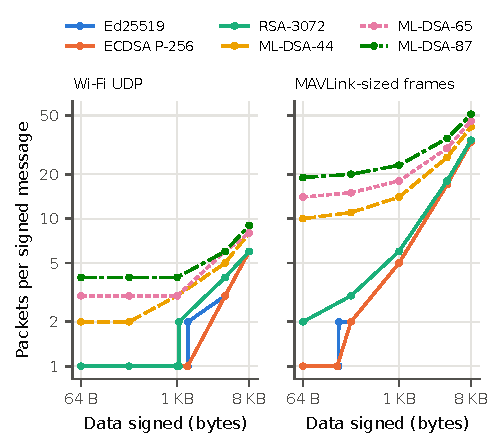
\includegraphics[width=0.62\textwidth]{fig6_link_packets.pdf}
\caption{Packets needed for one signed message as the data grows (measured, median of 20).}
\end{figure}

\begin{table}[H]
\centering\small
\begin{tabularx}{\textwidth}{@{}l RRR RRR@{}}
\toprule
 & \multicolumn{3}{c}{\textbf{64 bytes of data}} & \multicolumn{3}{c}{\textbf{1 KB of data}} \\
\cmidrule(lr){2-4}\cmidrule(l){5-7}
Algorithm & Wi-Fi packets & MAVLink frames & Bytes (Wi-Fi) & Wi-Fi packets & MAVLink frames & Bytes (Wi-Fi) \\
\midrule
Ed25519     & 1 & 1  & 168   & 1 & 5  & 1,128 \\
ECDSA P-256 & 1 & 1  & 175   & 1 & 5  & 1,135 \\
RSA-3072    & 1 & 2  & 488   & 1 & 6  & 1,448 \\
ML-DSA-44   & 2 & 10 & 2,544 & 3 & 14 & 3,524 \\
ML-DSA-65   & 3 & 14 & 3,453 & 3 & 18 & 4,413 \\
ML-DSA-87   & 4 & 19 & 4,791 & 4 & 23 & 5,751 \\
\bottomrule
\end{tabularx}
\caption{Packets and bytes for one signed authentication message (measured). Bytes are counted at
the IP level (headers included, Wi-Fi radio framing not included).}
\end{table}

In a small authentication (64 bytes of data), the signature is 38\% of the bytes with Ed25519, 41\%
with ECDSA, 79\% with RSA, and \textbf{95--97\% with ML-DSA}. The drone sends mostly signature, not
data.

\textbf{What Wireshark showed} (one authentication each, 64 bytes of data, MAVLink-sized frames;
times from the challenge leaving the laptop):

\begin{table}[H]
\centering\small
\begin{tabularx}{\textwidth}{@{}X X@{}}
\toprule
\textbf{Ed25519} & \textbf{ML-DSA-44} \\
\midrule
\texttt{0.00 ms \ CHALLENGE \ \ \ \ \ \ \ \ \ 72 B} &
\texttt{0.00 ms \ CHALLENGE \ \ \ \ \ \ \ \ \ \ 72 B} \\
\texttt{18.91 ms AUTH frame 1/1 \ 178 B} &
\texttt{44.51 ms AUTH frame 1/10 \ 293 B} \\
\texttt{19.98 ms RESULT \ \ \ \ \ \ \ \ \ \ \ \ 41 B} &
\texttt{\ \ \ \ \ \ \ \ \ ... frames 2/10 to 9/10 ...} \\
 & \texttt{44.87 ms AUTH frame 10/10 239 B} \\
 & \texttt{45.71 ms RESULT \ \ \ \ \ \ \ \ \ \ \ \ \ 41 B} \\
\bottomrule
\end{tabularx}
\caption{Packets of one authentication, taken from the Wireshark recording.}
\end{table}

% ---------------------------------------------------------------------------
\section{Wireshark screenshots}

These are taken from the recording of the final run, opened in Wireshark with our plug-in, which
names the messages (CHALLENGE, AUTH, RESULT; STAT lines are our own timing data, not part of the
authentication).

\begin{figure}[H]
\centering
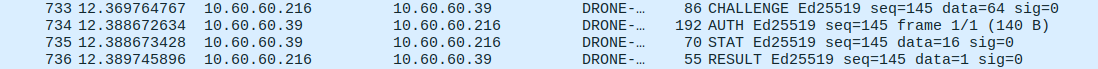
\includegraphics[width=\textwidth]{2_ed25519_mavlink_1_frame.png}\\[4pt]
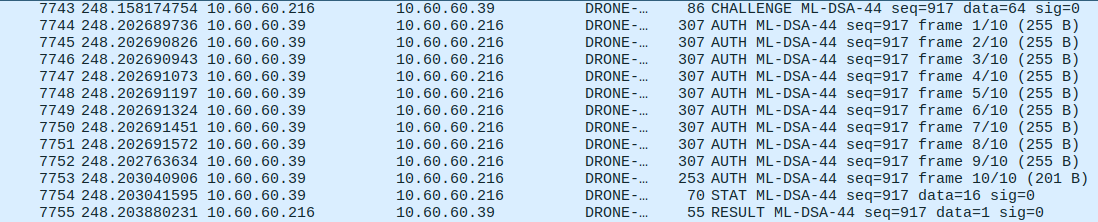
\includegraphics[width=\textwidth]{3_mldsa44_mavlink_10_frames.png}
\caption{The same authentication (64 bytes of data) in MAVLink-sized frames. Top: Ed25519, the
whole signed message (140 bytes) fits in 1 frame. Bottom: ML-DSA-44, the signed message needs 10
frames.}
\end{figure}

\begin{figure}[H]
\centering
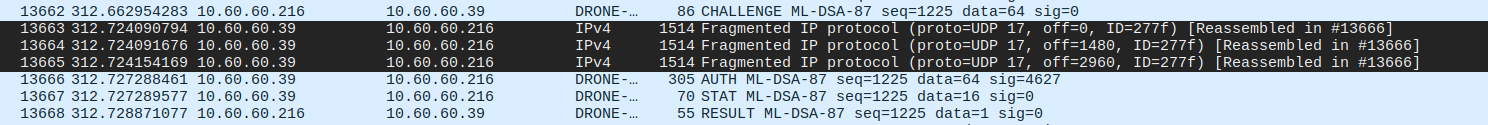
\includegraphics[width=\textwidth]{5_mldsa87_wifi_split_4_packets.png}
\caption{ML-DSA-87 on normal Wi-Fi: one signed message (64 bytes of data) is too big for one
packet, so the network splits it into 4 packets (3 pieces marked ``Fragmented IP protocol'' and the
last one, where Wireshark puts the message back together).}
\end{figure}

\begin{figure}[H]
\centering
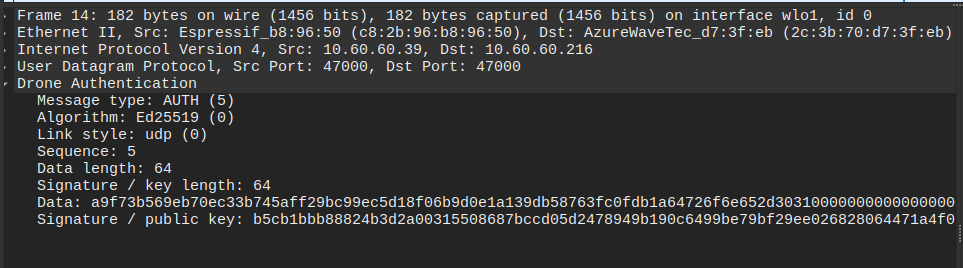
\includegraphics[width=0.85\textwidth]{6_ed25519_details_64B_signature.png}\\[4pt]
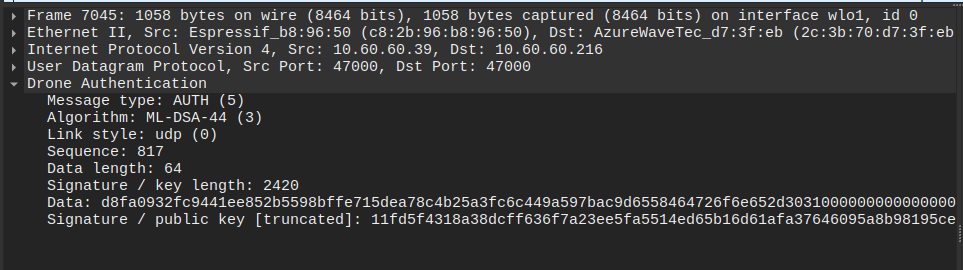
\includegraphics[width=0.85\textwidth]{7_mldsa44_details_2420B_signature.png}
\caption{Inside one signed message with 64 bytes of data. Top: Ed25519 adds a 64-byte signature.
Bottom: ML-DSA-44 adds a 2,420-byte signature.}
\end{figure}

More screenshots (the start-up messages, and ML-DSA-87 in 19 frames) are in
\texttt{results/e3/screenshots/}.

% ---------------------------------------------------------------------------
\section{Time for one authentication}

\begin{figure}[H]
\centering
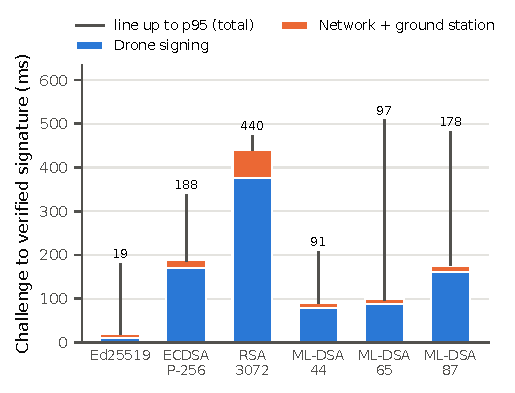
\includegraphics[width=0.62\textwidth]{fig7_link_time.pdf}
\caption{Where the time of one authentication goes (64 bytes of data, Wi-Fi; medians of 20). The
number is the median total; the line goes up to the 95th percentile.}
\end{figure}

\begin{table}[H]
\centering\small
\begin{tabularx}{0.9\textwidth}{@{}l RRRR@{}}
\toprule
Algorithm & Drone signing & Network + ground station & Total (median) & Total (p95) \\
\midrule
Ed25519     & 9.7\,ms   & 9.6\,ms  & 19.5\,ms  & 178.5\,ms \\
ECDSA P-256 & 169.9\,ms & 17.8\,ms & 187.7\,ms & 336.3\,ms \\
RSA-3072    & 376.0\,ms & 63.5\,ms & 440.2\,ms & 472.4\,ms \\
ML-DSA-44   & 78.9\,ms  & 11.5\,ms & 90.7\,ms  & 205.6\,ms \\
ML-DSA-65   & 86.9\,ms  & 11.4\,ms & 97.3\,ms  & 507.1\,ms \\
ML-DSA-87   & 160.2\,ms & 14.1\,ms & 177.7\,ms & 479.9\,ms \\
\bottomrule
\end{tabularx}
\caption{From the challenge leaving the ground station to the verified signature (64 bytes of data,
Wi-Fi). ``Network + ground station'' = total minus the drone's signing time. With 20 runs, the ML-DSA
signing medians are rough; Step 1 has the exact values from 1,000 runs.}
\end{table}

On Wi-Fi, the drone's signing is most of the time. The network adds about 10--20\,ms, and splitting
a message into several packets adds almost nothing, because Wi-Fi is fast: the 10 frames of an
ML-DSA-44 message left within 0.4\,ms.

\textbf{RSA's network part is larger (64\,ms).} Its delays fall into two groups, around 10--20\,ms
and around 80--100\,ms. About 100\,ms is the Wi-Fi ``beacon interval'', the period at which a hotspot
delivers data it has held back for a device it thinks is asleep. RSA keeps the drone's radio silent
the longest (about 430\,ms between messages), so this happens most often with RSA; it also happens
occasionally with the others (in their slowest 10\%). This is a property of the hotspot, not of the
algorithm, but it shows that slow signing can add up to one beacon interval on a real link.

% ---------------------------------------------------------------------------
\section{On a real drone radio, the packets cost much more time}

On Wi-Fi, extra packets are cheap. Drones often use a slower telemetry radio. Using the measured
message sizes and frame counts, this is how long sending one signed message would take on a
57.6\,kbit/s MAVLink radio (adding MAVLink 2's 12 bytes of header and checksum per frame):

\begin{table}[H]
\centering\small
\begin{tabularx}{0.9\textwidth}{@{}l RRR R@{}}
\toprule
 & \multicolumn{3}{c}{\textbf{64 bytes of data}} & \textbf{1 KB of data} \\
\cmidrule(lr){2-4}\cmidrule(l){5-5}
Algorithm & Frames & Bytes on the radio & Time & Time \\
\midrule
Ed25519     & 1  & 152   & 21\,ms  & 161\,ms \\
ECDSA P-256 & 1  & 160   & 22\,ms  & 162\,ms \\
RSA-3072    & 2  & 484   & 67\,ms  & 207\,ms \\
ML-DSA-44   & 10 & 2,616 & 363\,ms & 503\,ms \\
ML-DSA-65   & 14 & 3,553 & 493\,ms & 633\,ms \\
ML-DSA-87   & 19 & 4,931 & 685\,ms & 825\,ms \\
\bottomrule
\end{tabularx}
\caption{Calculated time to send one signed message over a 57.6\,kbit/s radio (bytes $\times$ 8 /
57,600), from the measured message sizes. Not measured on a real radio.}
\end{table}

On such a radio, one ML-DSA-44 authentication takes about 17 times longer to send than an Ed25519 one,
and the radio is busy all that time, so other telemetry has to wait.

% ---------------------------------------------------------------------------
\section{Reliability}

All 1,400 authentications in the final run were verified by the ground station, and none was lost
or rejected. An earlier run on the same set-up lost 3 of 1,400 (0.2\%); all messages that arrived
were valid. The ESP32's signal was very strong ($-8$\,dBm), because it was next to the phone.

% ---------------------------------------------------------------------------
\section{Notes and next steps}

\textbf{What we fixed on the way (so the numbers can be trusted).}
\begin{itemize}[nosep]
  \item The first recording kept only the first piece of each split message (a Wireshark filter
        issue). The filter was fixed, and the analysis now checks every message for missing pieces.
  \item In the second run, the laptop's Wi-Fi power saving was on. It delayed answers after a pause,
        mostly for RSA (about 87\,ms each). The final run was made with power saving off, and the
        ground station now warns if it is on.
\end{itemize}

\textbf{Limits.} One board, one phone hotspot, close range; 20 runs per point; the 57.6\,kbit/s
radio times are calculated, not measured.

\textbf{Next steps.} Step 4: sequence diagrams of the drone authentication. Step 5: the MPU6050
sensor, to see whether signing disturbs the sensor sampling.

The recording can be opened in Wireshark with readable names:
\begin{flushleft}\small\ttfamily
wireshark -X lua\_script:tools/wireshark/drone\_auth.lua \\
\hspace*{2em}results/e3/raw/link\_20261124\_210648/capture.pcapng
\end{flushleft}

\end{document}
